\documentclass[18pt, a3paper, landscape]{extarticle}
\usepackage{extsizes}
\usepackage{etoolbox}
\usepackage{environ}
\usepackage{xcolor} % [dvipsnames]
\usepackage{lscape, pdflscape}
\usepackage{pdfpages}

\usepackage{macros}

\usepackage{mdframed}
\mdfsetup{skipabove=0pt, skipbelow=0pt, frametitleaboveskip=0pt, frametitlebelowskip=0pt}

\usepackage{tcolorbox}
\tcbuselibrary{breakable}
\tcbset{nobeforeafter, breakable, colback=gray!10, colframe=gray!10}

\usepackage[landscape]{geometry}
\geometry{top=.1in,left=.1in,right=.1in,bottom=.1in}



\usepackage{array, makecell, multirow, tabularx}
% \renewcommand\theadfont{\normalsize\bfseries}
% \renewcommand{\arraystretch}{.0001}

\usepackage{multicol, booktabs, longtable}
\usepackage{extramarks, linegoal}
\usepackage{relsize, rotating}
\usepackage{enumerate, enumitem}
\setlist[itemize]{topsep=0pt,partopsep=0pt, parsep=0pt}
\setlist[description]{leftmargin=0pt}

\usepackage{wrapfig}
\usepackage{graphicx}
\graphicspath{{graphics/}}
\setkeys{Gin}{keepaspectratio}

\usepackage{caption}
\usepackage{subcaption}

\usepackage{algorithm}
\usepackage[noend]{algpseudocode}

%%%%%%%%%%%%%%%%%%%%%%%%%%%%%%%%%%%%%%%%%%%%%%%%%%%%%%%%%%%%%%%%%%%%%%%%%%%%%%%%

\pagestyle{empty}
\makeatletter
\renewcommand{\section}{\@startsection{section}{1}{0mm}%
                              {-1ex plus -.5ex minus -.2ex}%
                              {0.5ex plus .2ex}%x
                              {\normalfont\large\bfseries}}
\renewcommand{\subsection}{\@startsection{subsection}{2}{0mm}%
                              {-1explus -.5ex minus -.2ex}%
                              {0.5ex plus .2ex}%
                              {\normalfont\normalsize\bfseries}}
\renewcommand{\subsubsection}{\@startsection{subsubsection}{3}{0mm}%
                              {-1ex plus -.5ex minus -.2ex}%
                              {1ex plus .2ex}%
                              {\normalfont\small\bfseries}}
\makeatother

\setcounter{secnumdepth}{0}

% % https://tex.stackexchange.com/questions/47910/reduce-space-before-and-after-tabular-environment
% \setlength{\textfloatsep}{0.1cm}
% \addtolength{\parskip}{-0.5mm}
% \setlength{\intextsep}{0pt}
%
% % https://tex.stackexchange.com/questions/224987/how-to-decrease-space-above-and-below-displayed-equations
% \setlength\abovedisplayskip{0pt}
% \setlength\belowdisplayskip{0pt}
% \setlength\abovedisplayshortskip{0pt}
% \setlength\belowdisplayshortskip{0pt}
%
% \setlength\parskip{\baselineskip} % https://tex.stackexchange.com/questions/66533/implicit-newline-at-the-end-of-each-paragraph
\setlength{\parindent}{0pt}
\setlength{\parskip}{0pt plus 0.5ex}

\newcommand{\separator}{\smallskip \hrule height 2pt \smallskip}

%%%%%%%%%%%%%%%%%%%%%%%%%%%%%%%%%%%%%%%%%%%%%%%%%%%%%%%%%%%%%%%%%%%%%%%%%%%%%%%%

% \titlespacing{command}{left spacing}{before spacing}{after spacing}[right]
\usepackage{titlesec}
  \titlespacing{\section}{0pt}{0pt}{0pt}
  \titleformat{\section}
  {\color{blue}\normalfont\large\bfseries} % blue % Cerulean
  {\color{blue}\thesection}{1em}{} % blue % Cerulean

  \titlespacing{\subsection}{0pt}{0pt}{0pt}
  \titleformat{\subsection}
  {\color{cyan}\normalfont\normalsize\bfseries} % cyan % Turquoise
  {\color{cyan}\thesection}{1em}{} % cyan % Turquoise

  \titlespacing{\subsubsection}{0pt}{0pt}{0pt}
  \titleformat{\subsubsection}
  {\color{black}\normalfont\small\bfseries}
  {\color{black}\thesection}{1em}{}

%%%%%%%%%%%%%%%%%%%%%%%%%%%%%%%%%%%%%%%%%%%%%%%%%%%%%%%%%%%%%%%%%%%%%%%%%%%%%%%%
%%%%%%%%%%%%%%%%%%%%%%%%%%%%%%%%%%%%%%%%%%%%%%%%%%%%%%%%%%%%%%%%%%%%%%%%%%%%%%%%
\begin{document}
\raggedright
\footnotesize
\begin{multicols*}{3}
\setlength{\premulticols}{1pt}
\setlength{\postmulticols}{1pt}
\setlength{\multicolsep}{1pt}
\setlength{\columnsep}{2pt}
%%%%%%%%%%%%%%%%%%%%%%%%%%%%%%%%%%%%%%%%%%%%%%%%%%%%%%%%%%%%%%%%%%%%%%%%%%%%%%%%
%%%%%%%%%%%%%%%%%%%%%%%%%%%%%%%%%%%%%%%%%%%%%%%%%%%%%%%%%%%%%%%%%%%%%%%%%%%%%%%%

% Foundations
%\begin{tcolorbox}
\section{Statistics} \seperator
	\subsection{LLN}
		\begin{mdframed}%[backgroundcolor=gray!10, frametitleaboveskip=0pt, frametitlebelowskip=0pt, frametitle={}]
			\[
				\lim_{n \rightarrow \infinity} \abs{\frac{1}{n} \sum_{i=1}^{n} x_i - \Exp{x}} = 0
			\]
		\end{mdframed}
	\subsection{Unbiasedness}
		\begin{mdframed}%[backgroundcolor=gray!10, frametitleaboveskip=0pt, frametitlebelowskip=0pt, frametitle={}]
			\[
				\mathrm{Bias}_{\theta} = \Exp{\estimate{\theta}} - \theta = \Exp{\estimate{\theta} - \theta} = 0
			\]
		\end{mdframed}
	\subsection{Consistency}
		\begin{mdframed}%[backgroundcolor=gray!10, frametitleaboveskip=0pt, frametitlebelowskip=0pt, frametitle={}]
			\[
				\lim_{n \rightarrow \infinity} \Prob{ \abs{\widehat{X} - \frac{1}{n}\sum_{i=1}^{n} X_i} \leq \epsilon} = 1
			\]
		\end{mdframed}
	% \subsection{Hoeffding's Inequality}
	% 	\begin{mdframed}%[backgroundcolor=gray!10, frametitleaboveskip=0pt, frametitlebelowskip=0pt, frametitle={}]
	% 	\end{mdframed}
	% \subsection{Chebyshev's Inequality}
	% 	\begin{mdframed}%[backgroundcolor=gray!10, frametitleaboveskip=0pt, frametitlebelowskip=0pt, frametitle={}]
	% 	\end{mdframed}
	\subsection{Properties of Gaussians}
		\begin{mdframed}%[backgroundcolor=gray!10, frametitleaboveskip=0pt, frametitlebelowskip=0pt, frametitle={}]
			\[
				X \as \mathcal{N}(\mu,\, \sigma^2) \implies Y = aX + b \as \mathcal{N}(a\mu + b,\, a^2\sigma^2)
			\]
			\[
				X \as \mathcal{N}(\mu_x,\, \sigma^2_x),\,\qquad Y \as \mathcal{N}(\mu_y,\, \sigma^2_y),\,\quad \implies \quad Z = X + Y \as \mathcal{N}(\mu_x + \mu_y,\, \sigma^2_x + \sigma^2_y)
			\]
		\end{mdframed}
	% \subsection{Bayes Rule} % why not
	% 	\begin{mdframed}%[backgroundcolor=gray!10, frametitleaboveskip=0pt, frametitlebelowskip=0pt, frametitle={}]
	% 		% posterior, likelihood, prior, marginal
	% 		% unconditional version
	% 		% conditional version
	% 	\end{mdframed}
	% \subsection{Conjugate Prior}
	% 	\begin{mdframed}%[backgroundcolor=gray!10, frametitleaboveskip=0pt, frametitlebelowskip=0pt, frametitle={}]
	% 		% common conjugate priors...
	% 	\end{mdframed}
%\end{tcolorbox}

% % Foundations
% \section{Estimation} \seperator
% 	\subsection{MLE}
% 		\begin{mdframed}%[backgroundcolor=gray!10, frametitleaboveskip=0pt, frametitlebelowskip=0pt, frametitle={}]
% 		\end{mdframed}
% 	\subsection{MAP}
% 		\begin{mdframed}%[backgroundcolor=gray!10, frametitleaboveskip=0pt, frametitlebelowskip=0pt, frametitle={}]
% 		\end{mdframed}

% Foundations
%\begin{tcolorbox}
\section{Information Theory} \seperator
	\subsection{Information \qquad\qquad\qquad\qquad\qquad\qquad Information Gain}
		\begin{mdframed}%[backgroundcolor=gray!10, frametitleaboveskip=0pt, frametitlebelowskip=0pt, frametitle={}]
			\begin{minipage}{0.5\linewidth}
				\[
					\Information{S} = \log_2 \frac{1}{\Prob{S}}
				\]
			\end{minipage}%
			\vrule%
			\begin{minipage}{0.5\linewidth}
				\[
					\Information{Y,\, X_i} = \Entropy{Y} - \Entropy{Y \given X_i}
				\]
			\end{minipage}
		\end{mdframed}
	\subsection{Entropy}
		\begin{mdframed}%[backgroundcolor=gray!10, frametitleaboveskip=0pt, frametitlebelowskip=0pt, frametitle={}]
			\begin{align*}
		    \Entropy{S} &= \sum_{s \in \Set{S}} \Prob{S{=}s} \cdot \Information{S{=}s} = \sum_{s \in \Set{S}} \Prob{S{=}s} \log_2 \frac{1}{\Prob{S{=}s}} \\
		                &=\quad\! \Exp{\log_2 \sfrac{1}{\Prob{S{=}s}}}\qquad\quad\, =\ {-} \Exp{\log_2 \Prob{S{=}s}} \\
		                &= {-} \sum_{s \in \Set{S}} \Prob{S{=}s} \log_2 \Prob{S{=}s}
		  \end{align*}
		\end{mdframed}
%\end{tcolorbox}

% Foundations
%\begin{tcolorbox}
\section{Learning Theory} \seperator
	\subsection{PAC Learning}
		\begin{mdframed}%[backgroundcolor=gray!10, frametitleaboveskip=0pt, frametitlebelowskip=0pt, frametitle={}]
			\begin{minipage}{0.5\linewidth}%
				\[
					\Prob{\abs{\estimate{\theta} - \optimal{\theta}} \leq \epsilon} \geq 1 - \delta
				\]
			\end{minipage}%
			\vrule%
			\begin{minipage}{0.5\linewidth}%
				\[
					\Prob{\abs{\estimate{\theta} - \optimal{\theta}} > \epsilon} < \delta
				\]
			\end{minipage}
		\end{mdframed}
%\end{tcolorbox}

% Foundations
%\begin{tcolorbox}
\section{Decision Theory} \separator
	% \subsection{Common Loss Functions}
	% 	\begin{mdframed}%[backgroundcolor=gray!10, frametitleaboveskip=0pt, frametitlebelowskip=0pt, frametitle={}]
	% 	\end{mdframed}
	\subsection{Risk \qquad\qquad\qquad\qquad\qquad\qquad\qquad\qquad\quad Bayes Risk}
	\begin{mdframed}%[backgroundcolor=gray!10, frametitleaboveskip=0pt, frametitlebelowskip=0pt, frametitle={}]
		\begin{minipage}{0.5\linewidth}
			\[
				\mathrm{Risk}(f) = R(f) := \mathbb{E}_{(X,Y)} \Big[\loss \big(Y,\, f(X)\big)\Big]
			\]
		\end{minipage}%
		\qquad\vrule%
		\begin{minipage}{0.5\linewidth}
			\[
				R(f^*) \leq R(f),\ \forall\, f \in \mathcal{F}
			\]
		\end{minipage}
	\end{mdframed}
	\subsection{Bayes Optimal Rule}
		\begin{mdframed}%[backgroundcolor=gray!10, frametitleaboveskip=0pt, frametitlebelowskip=0pt, frametitle={}]
			\[
				f^{*}(P) = \argmin_{f} \mathbb{E}_{(X,Y) \as P} \Big[\loss \big(Y,\, f(X)\big)\Big]
			\]
		\end{mdframed}
	\subsection{Emperical Risk Minimization}
		\begin{mdframed}%[backgroundcolor=gray!10, frametitleaboveskip=0pt, frametitlebelowskip=0pt, frametitle={}]
			\[
				 \estimate{f}_{n} = \argmin_{f} \frac{1}{n} \sum_{i=1}^{n} \Big[\loss \big(Y_i,\, f(x_i)\big)\Big]\ \xrightarrow[n \rightarrow \infinity]{\quad\text{  LNN  }\quad}\ \argmin_{f} \mathbb{E}_{(X,\,Y)} \Big[\loss \big(Y,\, f(X)\big)\Big]
			\]
		\end{mdframed}
%\end{tcolorbox}

\columnbreak

% Foundations
%\begin{tcolorbox}
\section{Risk} \separator
	\subsection{True Risk \qquad\qquad\qquad\qquad\ Emperical Risk \qquad\qquad\quad Excess Risk}
		\begin{mdframed}%[backgroundcolor=gray!10, frametitleaboveskip=0pt, frametitlebelowskip=0pt, frametitle={}]
			\begin{minipage}{0.3\linewidth}
				\[
					R(f) := \mathbb{E}_{(X,Y)} \Big[\loss \big(f(X),\, Y\big)\Big]
				\]
			\end{minipage}%
			\hfill\vrule\hfill%
			\begin{minipage}{0.35\linewidth}
				\[
					\widehat{R}_{\mathcal{D}}(f) := \frac{1}{\Card{\mathcal{D}}} \sum_{i \in \mathcal{D}} \Big[\loss \big(f(X_i),\, Y_i\big)\Big]
				\]
			\end{minipage}%
			\hfill\vrule\hfill%
			\begin{minipage}{0.25\linewidth}
				\[
					\Exp{R(\estimate{f}_{n})} - R(\optimal{f})
				\]
			\end{minipage}
		\end{mdframed}
	\subsection{Structural Risk}
		\begin{mdframed}%[backgroundcolor=gray!10, frametitleaboveskip=0pt, frametitlebelowskip=0pt, frametitle={}]
			\begin{minipage}{0.35\linewidth}
				\begin{align*}
					& \abs{R(f) - \widehat{R}_{n}(f)} \leq C(f) & \forall\, f \in \mathcal{F} \\
					& R(f) \leq \widehat{R}_{n}(f) + C(f) & \forall\, f \in \mathcal{F}\\
				\end{align*}
				Use \(\widehat{R}_{n}(\estimate{f}_{n}) + C(\estimate{f}_{n})\) as a \textit{pessimistic} estimate of true risk.
			\end{minipage}%
			\begin{minipage}{0.65\linewidth}
				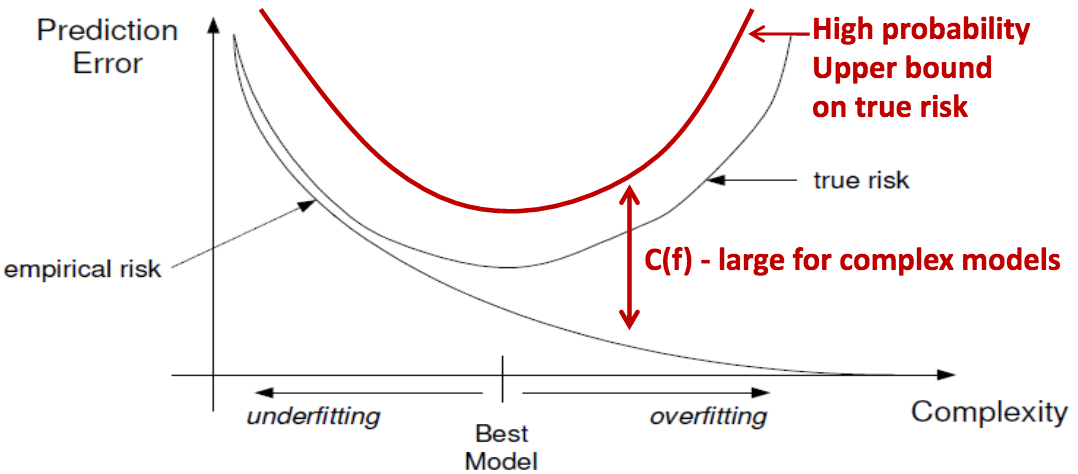
\includegraphics[width=\linewidth]{structural_risk_curve.png}
			\end{minipage}
		\end{mdframed}
%\end{tcolorbox}

% Foundations
%\begin{tcolorbox}
\section{Risk Estimation}
	\subsection{Bias--Variance Tradeoff}
		\begin{mdframed}%[backgroundcolor=gray!10, frametitleaboveskip=0pt, frametitlebelowskip=0pt, frametitle={}]
			\begin{minipage}{0.3\linewidth}
				\begin{align*}
					\mathrm{Bias} &= \Exp{f(X)} - \optimal{f}(X) \\
					\mathrm{Variance} &= \Exp{{(f(X) - \Exp{f(X))}^2}} \\
					\mathrm{Bias}^2 &+ \mathrm{Variance} = \\
					& \Exp{{(f(X) - \optimal{f}(X))}^2}
				\end{align*}
			\end{minipage}%
			\hfill%
			\begin{minipage}{0.3\linewidth}
				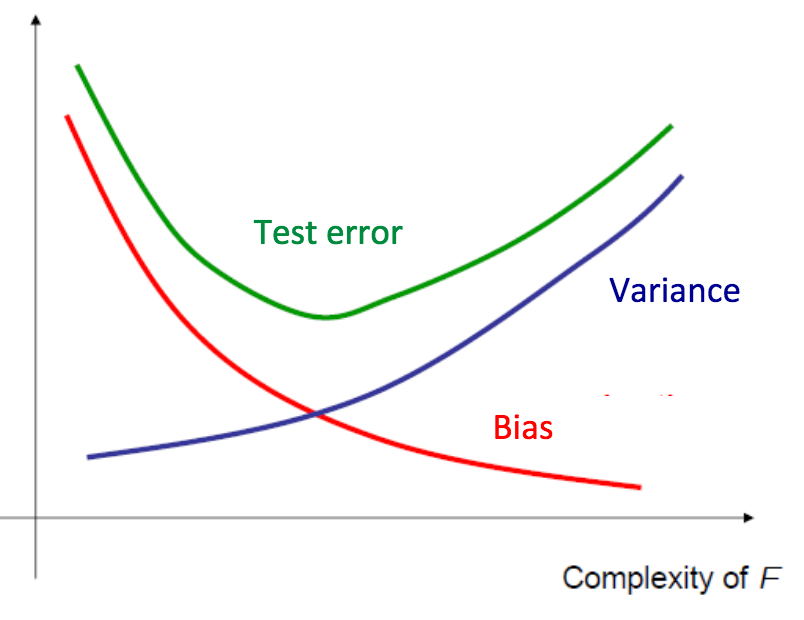
\includegraphics[width=\linewidth]{bias_vs_variance_error.png}
			\end{minipage}%
			\hfill%
			\begin{minipage}{0.3\linewidth}
				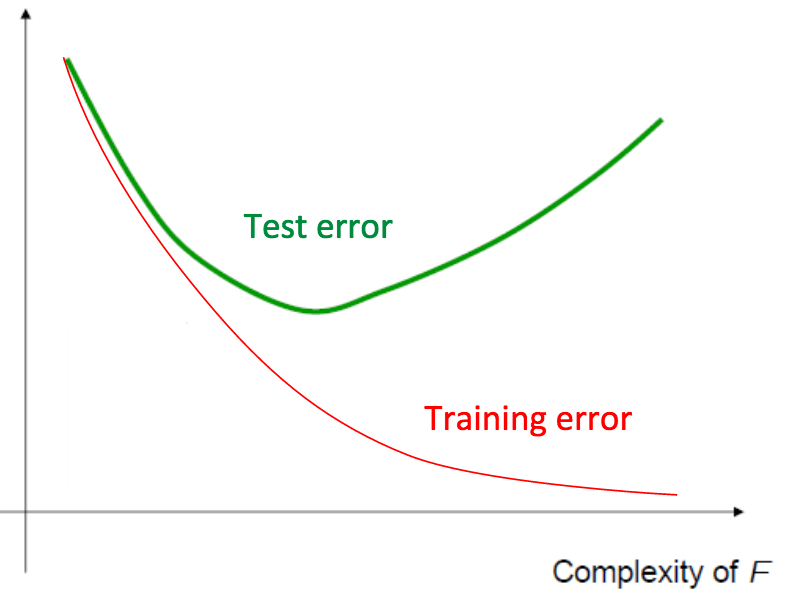
\includegraphics[width=\linewidth]{test_vs_train_error.png}
			\end{minipage}
		\end{mdframed}
	\subsection{K--Fold CV \qquad\qquad\qquad\quad LOO CV \qquad\qquad\qquad Random Subsampling}
		\begin{mdframed}%[backgroundcolor=gray!10, frametitleaboveskip=0pt, frametitlebelowskip=0pt, frametitle={}]
			% width=0.95\linewidth,totalheight=0.95\textheight,keepaspectratio
			\begin{minipage}{0.3\linewidth}
				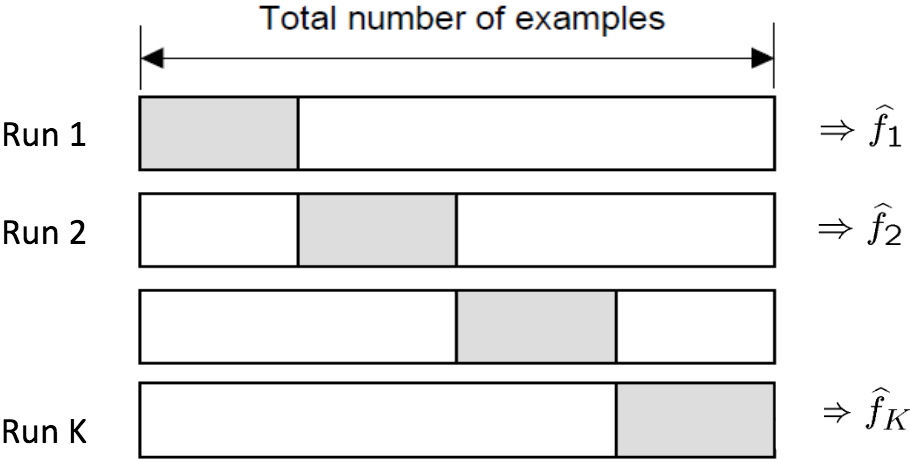
\includegraphics[width=\linewidth]{K_fold_cross_validation.png}
			\end{minipage}%
			\hfill%
			\begin{minipage}{0.3\linewidth}
				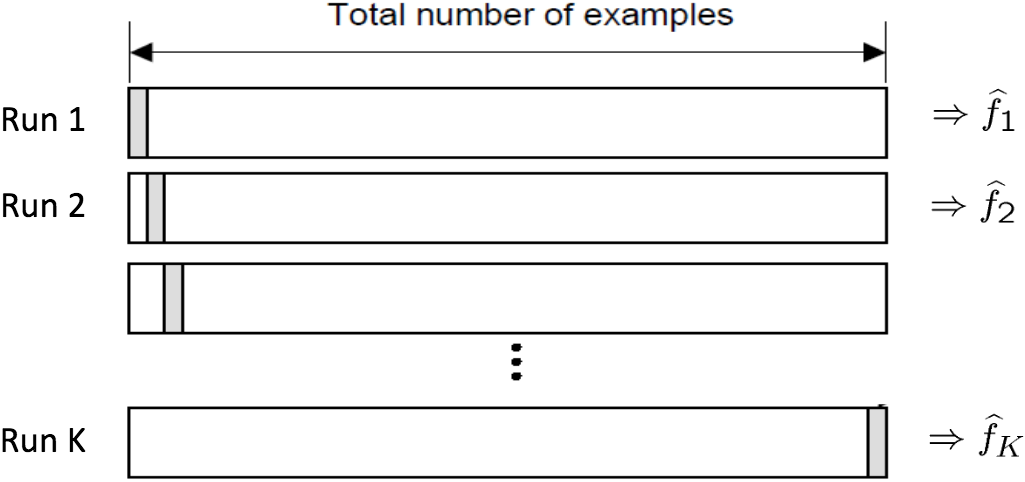
\includegraphics[width=\linewidth]{LOO_cross_validation.png}
			\end{minipage}%
			\hfill%
			\begin{minipage}{0.3\linewidth}
				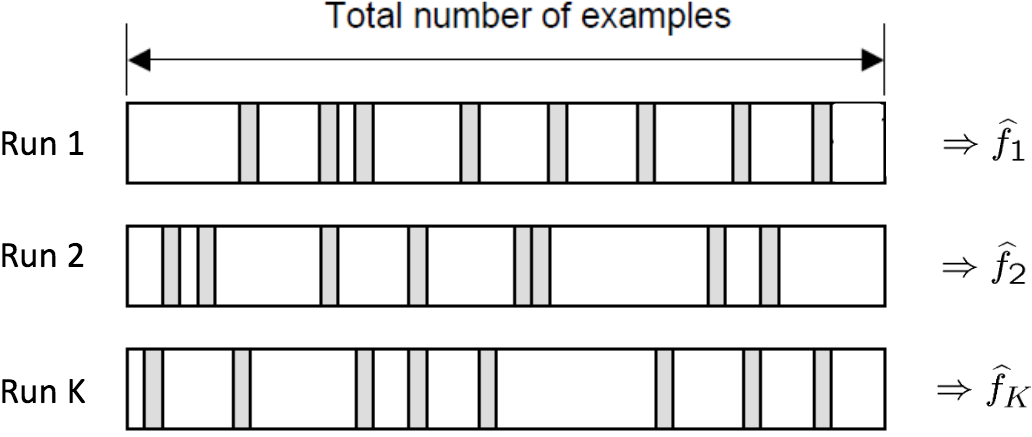
\includegraphics[width=\linewidth]{random_subsampling.png}
			\end{minipage}
		\end{mdframed}
	\subsection{Hold--out Method}
		\begin{mdframed}%[backgroundcolor=gray!10, frametitleaboveskip=0pt, frametitlebelowskip=0pt, frametitle={}]
			\begin{minipage}{0.4\linewidth}
				\begin{enumerate}[leftmargin=*]
					\item split into two sets
					\item use \(\mathcal{D}_{T}\) to train a predictor \(\estimate{f}_{\mathcal{D}_{T}}\)
					\item use \(\mathcal{D}_{V}\) to evaluate the predictor,
				\end{enumerate}
				\[
					\widehat{R}_{\mathcal{D}_{V}}(\estimate{f}_{\mathcal{D}_{T}})
				\]
			\end{minipage}%
			\hfill\vrule\hfill%
			\begin{minipage}{0.50\linewidth}
				\[
					\mathcal{D} = \Set{(X_i,\, Y_i)}_{i=1}^{n}
				\]
				\[
					\downarrow
				\]
				\[
					\underbrace{\mathcal{D}_{T} = \Set{(X_i,\, Y_i)}_{i=1}^{m}}_{\text{training set}}
					\qquad
					\underbrace{\mathcal{D}_{V} = \Set{(X_i,\, Y_i)}_{i=m+1}^{n}}_{\text{holdout set}}
				\]
			\end{minipage}
		\end{mdframed}
	\subsection{Estimating True Risk}
		\begin{mdframed}%[backgroundcolor=gray!10, frametitleaboveskip=0pt, frametitlebelowskip=0pt, frametitle={}]
			\begin{minipage}{0.5\linewidth}
				Estimate the error of a predictor on \(n\) data points.\\
				If K is large (close to \(n)\), bias of error estimate is small since each training set has close to \(n\) data points.\\
				However, variance of error estiamtes is high since each validation set has fewer data points and \(\widehat{R}_{V_{k}}\) might deviate a lot from the mean.\\
				\[
					\text{Error estimate} = \frac{1}{K} \sum_{k=1}^{K} \widehat{R}_{V_{k}} (\estimate{f}_{T_{k}})
				\]
			\end{minipage}%
			\begin{minipage}{0.5\linewidth}
				\hfill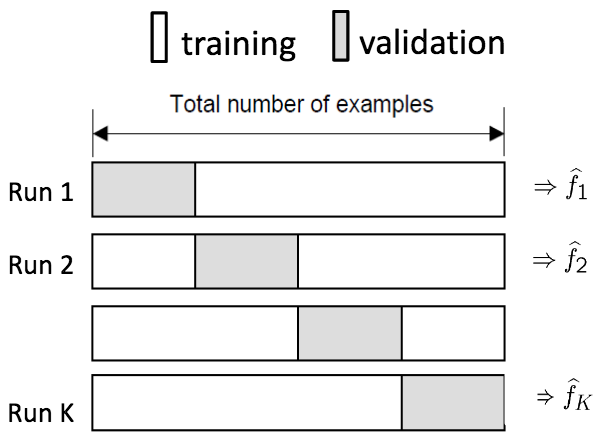
\includegraphics[width=0.85\linewidth]{estimating_true_risk.png}
			\end{minipage}
		\end{mdframed}
%\end{tcolorbox}

% Foundations
%\begin{tcolorbox}
\section{Risk Minimization} \separator
	\subsection{Emperical Risk Minimization \qquad\qquad\qquad Structural Risk Minimization}
		\begin{mdframed}%[backgroundcolor=gray!10, frametitleaboveskip=0pt, frametitlebelowskip=0pt, frametitle={}]
			\begin{minipage}{0.5\linewidth}
				\[
					\widehat{f_n} = \argmin_{f} \frac{1}{n} \sum_{i=1}^{n} \bigg[\loss \Big( Y_i,\, f(x_i) \Big) \bigg]
				\]
			\end{minipage}%
			\quad\vrule\quad%
			\begin{minipage}{0.5\linewidth}
				\[
					\estimate{f}_{n} = \argmin_{f \in \mathcal{F}} \Big\lbrack \widehat{R}_{n}(f) + \lambda C(f) \Big\rbrack
				\]
			\end{minipage}
		\end{mdframed}
%\end{tcolorbox}

\columnbreak

% Foundations
%\begin{tcolorbox}
\section{Overfitting} \separator
	\begin{mdframed}%[backgroundcolor=gray!10, frametitleaboveskip=0pt, frametitlebelowskip=0pt, frametitle={}]
		\begin{minipage}{0.3\linewidth}
			discrepency between emperical risk and true risk,\\ so emperical risk is no longer a good indicator of true risk
		\end{minipage}%
		\begin{minipage}{0.7\linewidth}
			\begin{center}
        \centering
        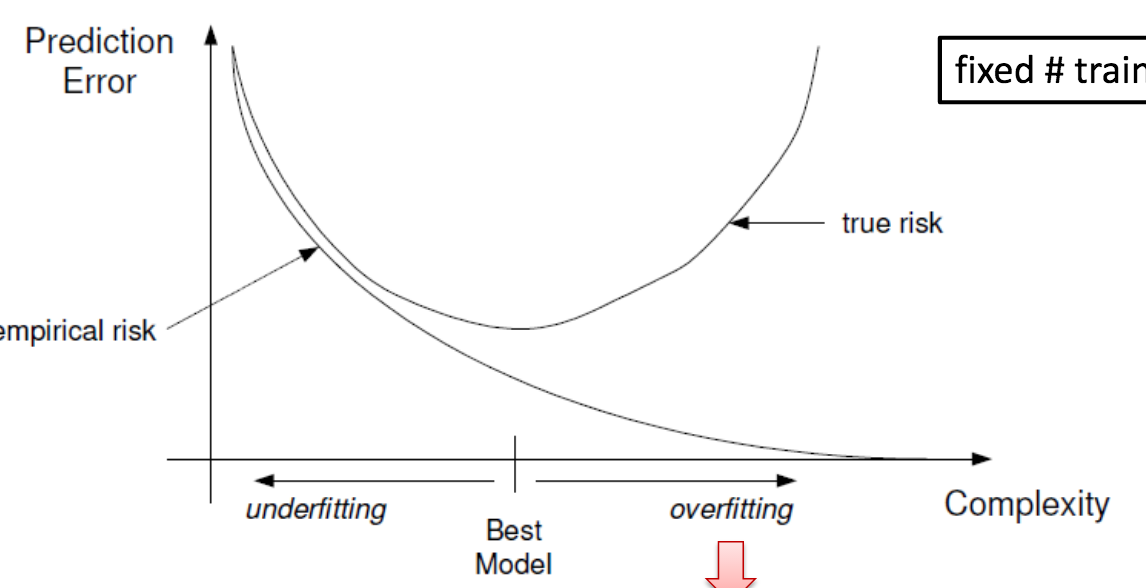
\includegraphics[width=\linewidth]{overfitting.png}
      \end{center}
		\end{minipage}
	\end{mdframed}
%\end{tcolorbox}

% Foundations
%\begin{tcolorbox}
\section{Regularization} \separator
	\subsection{Complexity Regularization}
		\begin{mdframed}%[backgroundcolor=gray!10, frametitleaboveskip=0pt, frametitlebelowskip=0pt, frametitle={}]
			\begin{minipage}{0.5\linewidth}%
				\[
					\estimate{f}_{n} = \argmin_{f \in \mathcal{F}} \Big\lbrace \widehat{R}_{n}(f) + \lambda C(f) \Big\rbrace
				\]
			\end{minipage}%
			\begin{minipage}{0.5\linewidth}%
				\begin{align*}
					C(f) &\ \colon\ \text{bound on deviation from true risk}\\
					\lambda &\ \colon\ \text{regularization penality}
				\end{align*}
			\end{minipage}
		\end{mdframed}
	\subsection{Information Criteria}
		\begin{mdframed}%[backgroundcolor=gray!10, frametitleaboveskip=0pt, frametitlebelowskip=0pt, frametitle={}]
			AIC (Akiake IC) \quad \(C(f) = \#\, parameters\)\\
			\indent Allows \(\#\) parameters to be infinite as \(\#\) training data \(n\) becomes large
		\end{mdframed}
		\begin{mdframed}%[backgroundcolor=gray!10, frametitleaboveskip=0pt, frametitlebelowskip=0pt, frametitle={}]
			BIC (Bayesian IC) \quad \(C(f) = \#\, parameters * \log n\)\\
			\indent Penalizes complex models more heavily -- limits complexity of models as \(\#\) training data \(n\) becomes large
		\end{mdframed}
%\end{tcolorbox}

% Foundations
%\begin{tcolorbox}
\section{Model Selection} \separator
	\begin{mdframed}%[backgroundcolor=gray!10, frametitleaboveskip=0pt, frametitlebelowskip=0pt, frametitle={}]
		\begin{itemize}
			\item define a finite set of model classes
			\item estimate true risk for each model class
			\item select model class with lowest estimated true risk
		\end{itemize}
	\end{mdframed}
	\begin{mdframed}%[backgroundcolor=gray!10, frametitleaboveskip=0pt, frametitlebelowskip=0pt, frametitle={}]
		Model classes \(\Set{\mathcal{F}_{\lambda}}\) of increasing complexity \(\mathcal{F}_{1} < \mathcal{F}_{2} < \ldots\)
		\[\min_{\lambda} \min_{f \in \mathcal{F}_{\lambda}} J(f,\, \lambda)\]
		\begin{itemize}
			\item given \(\lambda\) estimate \(\estimate{f}_{\lambda}\) using \textit{emperical / structural / complexity regularized} risk minimization
			\item select \(\lambda\) for which \(\estimate{f}_{\lambda}\) has minimum true risk estimated using \textit{cross--validation / hold--out / information criteria}
		\end{itemize}
	\end{mdframed}
%\end{tcolorbox}

% Foundations
%\begin{tcolorbox}
\section{Generalization Error} \separator
	\subsection{Terms}
		\begin{mdframed}%[backgroundcolor=gray!10, frametitleaboveskip=0pt, frametitlebelowskip=0pt, frametitle={}]
			\begin{minipage}{0.5\linewidth}
				\begin{gather*}
					\text{estimated predictor} := \estimate{f}_{n} \\
					\text{risk of estimated predictor} := R(\estimate{f}_{n}) \\
					\text{expected risk} := \Exp{R(\estimate{f}_{n})}
				\end{gather*}
			\end{minipage}%
			\begin{minipage}{0.5\linewidth}
				\begin{gather*}
					\text{optimal predictor} := \optimal{f} \\
					\text{risk of optimal predictor} := R(\optimal{f}) \\
					\text{excess risk} := \Exp{R(\estimate{f}_{n})} - R(\optimal{f})
				\end{gather*}
			\end{minipage}
		\end{mdframed}
	\subsection{True Risk Decomposition}
		\begin{mdframed}%[backgroundcolor=gray!10, frametitleaboveskip=0pt, frametitlebelowskip=0pt, frametitle={}]
		\[
			\Exp{R(\estimate{f}_{n})} - \optimal{R} = \underbrace{\Big\lparen \Exp{R(\estimate{f}_{n})} - \inf_{f \in \mathcal{F}} R(f) \Big\rparen}_{\text{estimation error}} + \underbrace{\Big\lparen \inf_{f \in \mathcal{F}} R(f) - \optimal{R} \Big\rparen}_{\text{approximation error}}
		\]
		\textit{Estimation Error} : due to randomness of training data \\
		\textit{Approximation Error} : due to restriction of model class \\
		\end{mdframed}
		\begin{mdframed}%[backgroundcolor=gray!10, frametitleaboveskip=0pt, frametitlebelowskip=0pt, frametitle={}]
			\begin{minipage}{0.5\linewidth}
				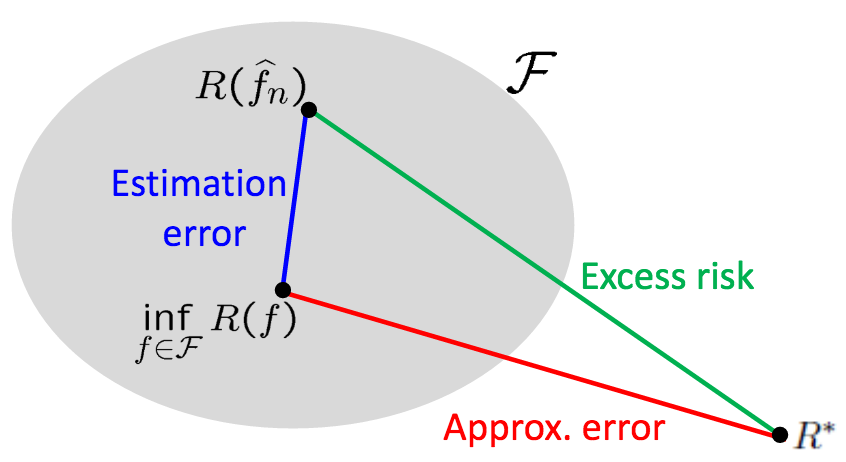
\includegraphics[width=0.95\linewidth]{true_risk_triangle.png}
			\end{minipage}%
			\begin{minipage}{0.5\linewidth}
				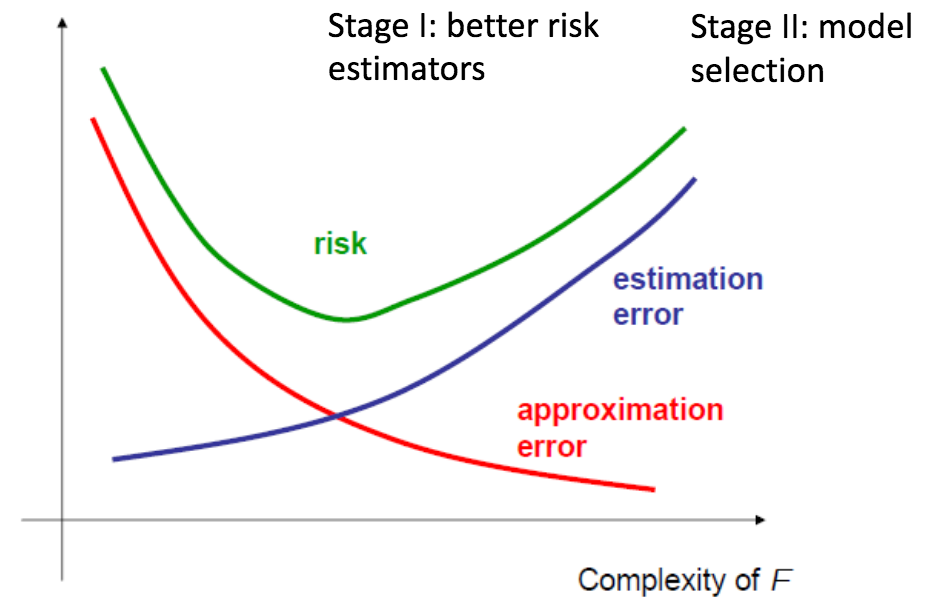
\includegraphics[width=0.5\linewidth]{true_risk_curve.png}
			\end{minipage}
		\end{mdframed}
%\end{tcolorbox}

\clearpage

% Parametric Models
%\begin{tcolorbox}
\section{Regression} \separator
	\subsection{Linear Regression}
		\begin{mdframed}%[backgroundcolor=gray!10, frametitleaboveskip=0pt, frametitlebelowskip=0pt, frametitle={}]
			\vspace{10mm}
		\end{mdframed}
		\begin{mdframed}%[backgroundcolor=gray!10, frametitleaboveskip=0pt, frametitlebelowskip=0pt, frametitle={}]
			\vspace{20mm}
		\end{mdframed}
	\subsection{Ridge Regression}
		\begin{mdframed}%[backgroundcolor=gray!10, frametitleaboveskip=0pt, frametitlebelowskip=0pt, frametitle={}]
			\[
				\estimate{\theta}_{\map}\argmin_{\theta} \sum_{i=1}^{n} {(Y_i - X_i \theta)}^2 + \lambda \norm{\theta}_{2}^{2}
			\]
		\end{mdframed}
		\begin{mdframed}%[backgroundcolor=gray!10, frametitleaboveskip=0pt, frametitlebelowskip=0pt, frametitle={}]
			\vspace{20mm}
		\end{mdframed}
	\subsection{Lasso Regression}
		\begin{mdframed}%[backgroundcolor=gray!10, frametitleaboveskip=0pt, frametitlebelowskip=0pt, frametitle={}]
			\[
				\estimate{\theta}_{\map}\argmin_{\theta} \sum_{i=1}^{n} {(Y_i - X_i \theta)}^2 + \lambda \norm{\theta}_{1}
			\]
		\end{mdframed}
		\begin{mdframed}%[backgroundcolor=gray!10, frametitleaboveskip=0pt, frametitlebelowskip=0pt, frametitle={}]
			\vspace{15mm}
		\end{mdframed}
	\subsection{Polynomial Regression}
		\begin{mdframed}%[backgroundcolor=gray!10, frametitleaboveskip=0pt, frametitlebelowskip=0pt, frametitle={}]
			\vspace{10mm}
		\end{mdframed}
		\begin{mdframed}%[backgroundcolor=gray!10, frametitleaboveskip=0pt, frametitlebelowskip=0pt, frametitle={}]
			\vspace{20mm}
		\end{mdframed}
%\end{tcolorbox}

% Parametric Models
%\begin{tcolorbox}
\section{Classification} \separator
	\subsection{Logistic Regression}
		\begin{mdframed}%[backgroundcolor=gray!10, frametitleaboveskip=0pt, frametitlebelowskip=0pt, frametitle={}]
			\vspace{10mm}
		\end{mdframed}
		\begin{mdframed}%[backgroundcolor=gray!10, frametitleaboveskip=0pt, frametitlebelowskip=0pt, frametitle={}]
			\vspace{20mm}
		\end{mdframed}
	\subsection{Naive Bayes}
		\begin{mdframed}%[backgroundcolor=gray!10, frametitleaboveskip=0pt, frametitlebelowskip=0pt, frametitle={}]
			\vspace{10mm}
		\end{mdframed}
		\begin{mdframed}%[backgroundcolor=gray!10, frametitleaboveskip=0pt, frametitlebelowskip=0pt, frametitle={}]
			\vspace{20mm}
		\end{mdframed}

\vfill\null
\columnbreak

	\subsection{Boosting}
		\begin{mdframed}%[backgroundcolor=gray!10, frametitleaboveskip=0pt, frametitlebelowskip=0pt, frametitle={}]
			\vspace{10mm}
		\end{mdframed}
		\begin{mdframed}%[backgroundcolor=gray!10, frametitleaboveskip=0pt, frametitlebelowskip=0pt, frametitle={}]
			\vspace{20mm}
		\end{mdframed}
	\subsection{Decision Trees}
		\begin{mdframed}%[backgroundcolor=gray!10, frametitleaboveskip=0pt, frametitlebelowskip=0pt, frametitle={}]
			\begin{align*}
		    \argmax_{X_i} \Big\lbrack \Entropy{Y} &- \Entropy{Y \given X_i} \Big\rbrack = \argmin_{X_i} \Entropy{Y \given X_i} \\
		      &= \argmin_{X_i} \sum_{x \in \Set{X_i}} \Big\lbrack \Prob{X_i{=}x} \Entropy{Y \given X_i{=}x} \Big\rbrack \\
		      &= \argmin_{X_i} {-} \sum_{x \in \Set{X_i}} \bigg\lbrack \Prob{X_i{=}x} \sum_{y \in \Set{Y}} \Big\lbrack \Prob{Y{=} \given X_i{=}x} \log_2 \Prob{Y{=}y \given X_i{=}x} \Big\rbrack \bigg\rbrack
		  \end{align*}
		\end{mdframed}
		\begin{mdframed}%[backgroundcolor=gray!10, frametitleaboveskip=0pt, frametitlebelowskip=0pt, frametitle={}]
			\vspace{20mm}
		\end{mdframed}
	\subsection{Support Vector Machines}
		\begin{mdframed}%[backgroundcolor=gray!10, frametitleaboveskip=0pt, frametitlebelowskip=0pt, frametitle={}]
			\vspace{10mm}
		\end{mdframed}
		\begin{mdframed}%[backgroundcolor=gray!10, frametitleaboveskip=0pt, frametitlebelowskip=0pt, frametitle={}]
			\vspace{30mm}
		\end{mdframed}
%\end{tcolorbox}

% Parametric Models
%\begin{tcolorbox}
\section{Deep Learning} \separator
	\subsection{Common Activation Functions}
		\begin{mdframed}%[backgroundcolor=gray!10, frametitleaboveskip=0pt, frametitlebelowskip=0pt, frametitle={}]
			\vspace{20mm}
		\end{mdframed}
	\subsection{Backpropagation}
		\begin{mdframed}%[backgroundcolor=gray!10, frametitleaboveskip=0pt, frametitlebelowskip=0pt, frametitle={}]
			\vspace{35mm}
		\end{mdframed}
	\subsection{Gradient Descent}
		\begin{mdframed}%[backgroundcolor=gray!10, frametitleaboveskip=0pt, frametitlebelowskip=0pt, frametitle={}]
			\vspace{35mm}
		\end{mdframed}
	\subsection{Perceptron}
		\begin{mdframed}%[backgroundcolor=gray!10, frametitleaboveskip=0pt, frametitlebelowskip=0pt, frametitle={}]
			\vspace{15mm}
		\end{mdframed}
	\subsection{MLP}
		\begin{mdframed}%[backgroundcolor=gray!10, frametitleaboveskip=0pt, frametitlebelowskip=0pt, frametitle={}]
			\vspace{15mm}
		\end{mdframed}
	\subsection{CNN}
		\begin{mdframed}%[backgroundcolor=gray!10, frametitleaboveskip=0pt, frametitlebelowskip=0pt, frametitle={}]
			\vspace{15mm}
		\end{mdframed}
	\subsection{RNN}
		\begin{mdframed}%[backgroundcolor=gray!10, frametitleaboveskip=0pt, frametitlebelowskip=0pt, frametitle={}]
			\vspace{15mm}
		\end{mdframed}
	\subsection{LSTM}
		\begin{mdframed}%[backgroundcolor=gray!10, frametitleaboveskip=0pt, frametitlebelowskip=0pt, frametitle={}]
			\vspace{15mm}
		\end{mdframed}
%\end{tcolorbox}

% Non--Parametric Models
%\begin{tcolorbox}
\section{Clustering} \separator % Supervised Learning
	\subsection{KNN}
		\begin{mdframed}%[backgroundcolor=gray!10, frametitleaboveskip=0pt, frametitlebelowskip=0pt, frametitle={}]
			\vspace{10mm}
		\end{mdframed}
		\begin{mdframed}%[backgroundcolor=gray!10, frametitleaboveskip=0pt, frametitlebelowskip=0pt, frametitle={}]
			\vspace{15mm}
		\end{mdframed}
	\subsection{Kernel Regression}
		\begin{mdframed}%[backgroundcolor=gray!10, frametitleaboveskip=0pt, frametitlebelowskip=0pt, frametitle={}]
			\vspace{10mm}
		\end{mdframed}
		\begin{mdframed}%[backgroundcolor=gray!10, frametitleaboveskip=0pt, frametitlebelowskip=0pt, frametitle={}]
			\vspace{15mm}
		\end{mdframed}
	\subsection{Kernel Trick}
		\begin{mdframed}%[backgroundcolor=gray!10, frametitleaboveskip=0pt, frametitlebelowskip=0pt, frametitle={}]
			\vspace{15mm}
		\end{mdframed}
%\end{tcolorbox}

%%%%%%%%%%%%%%%%%%%%%%%%%%%%%%%%%%%%%%%%%%%%%%%%%%%%%%%%%%%%%%%%%%%%%%%%%%%%%%%%
%%%%%%%%%%%%%%%%%%%%%%%%%%%%%%%%%%%%%%%%%%%%%%%%%%%%%%%%%%%%%%%%%%%%%%%%%%%%%%%%
\end{multicols*}
\end{document}
%%%%%%%%%%%%%%%%%%%%%%%%%%%%%%%%%%%%%%%%%%%%%%%%%%%%%%%%%%%%%%%%%%%%%%%%%%%%%%%%
%%%%%%%%%%%%%%%%%%%%%%%%%%%%%%%%%%%%%%%%%%%%%%%%%%%%%%%%%%%%%%%%%%%%%%%%%%%%%%%%
